\chapter{結論}

本研究は、遠隔型自動運転システムのユーザビリティに関して、
シミュレーションによる遠隔型自動運転における体感速度のモデルの提案と、
LiDARのみのSLAMによる自律移動システムとして、
手動・自動運転引継ぎシステムの実機開発と、
開発したシステムの評価をまとめたものである。
図\ref{auto:soukatsu}、\ref{auto:taikan_tokusei_final}に本論文で提案した
手動・自動運転引継ぎシステムとその構成要素の概略、体感速度モデルを示し、
本論文の内容を総括する。

\begin{figure}[h]
  \begin{center}
  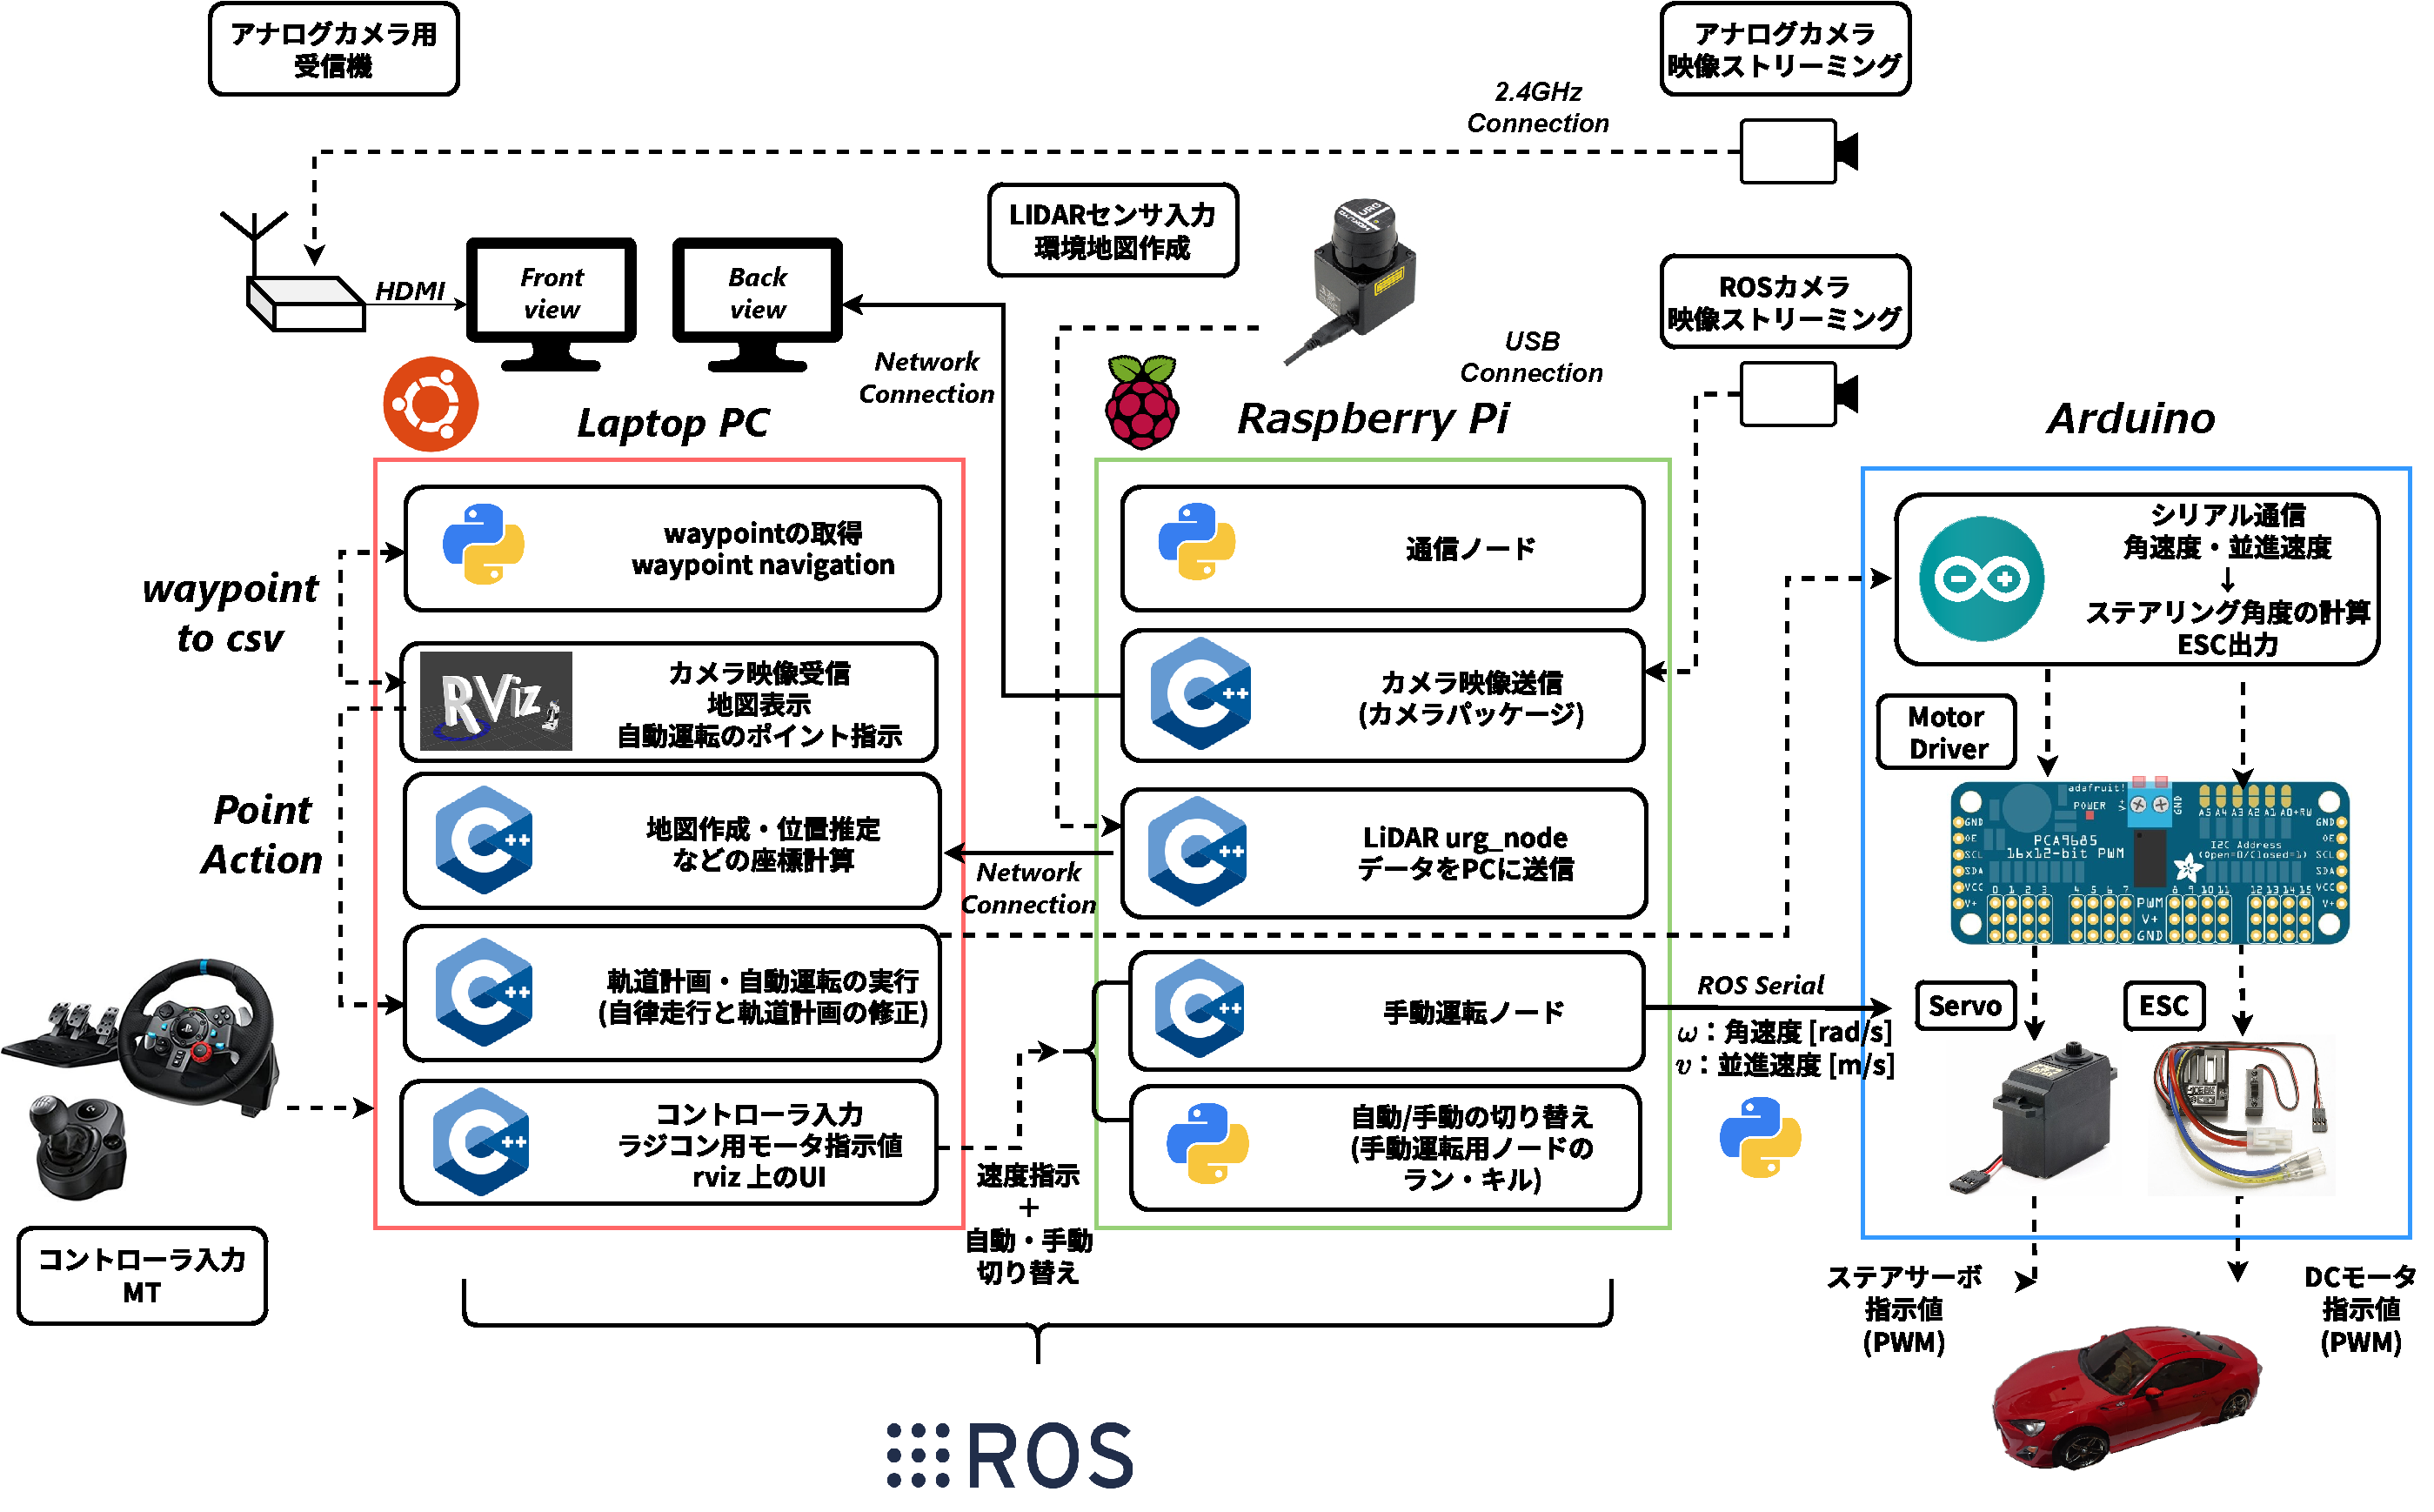
\includegraphics[width=\linewidth]{img/auto_2.pdf}
  \caption{手動・自動運転引継ぎシステム}
  \label{auto:soukatsu}
  \end{center}
\end{figure}

\begin{figure}[h]
  \begin{center}
    \subfigure[視野角と体感速度の特性]{
    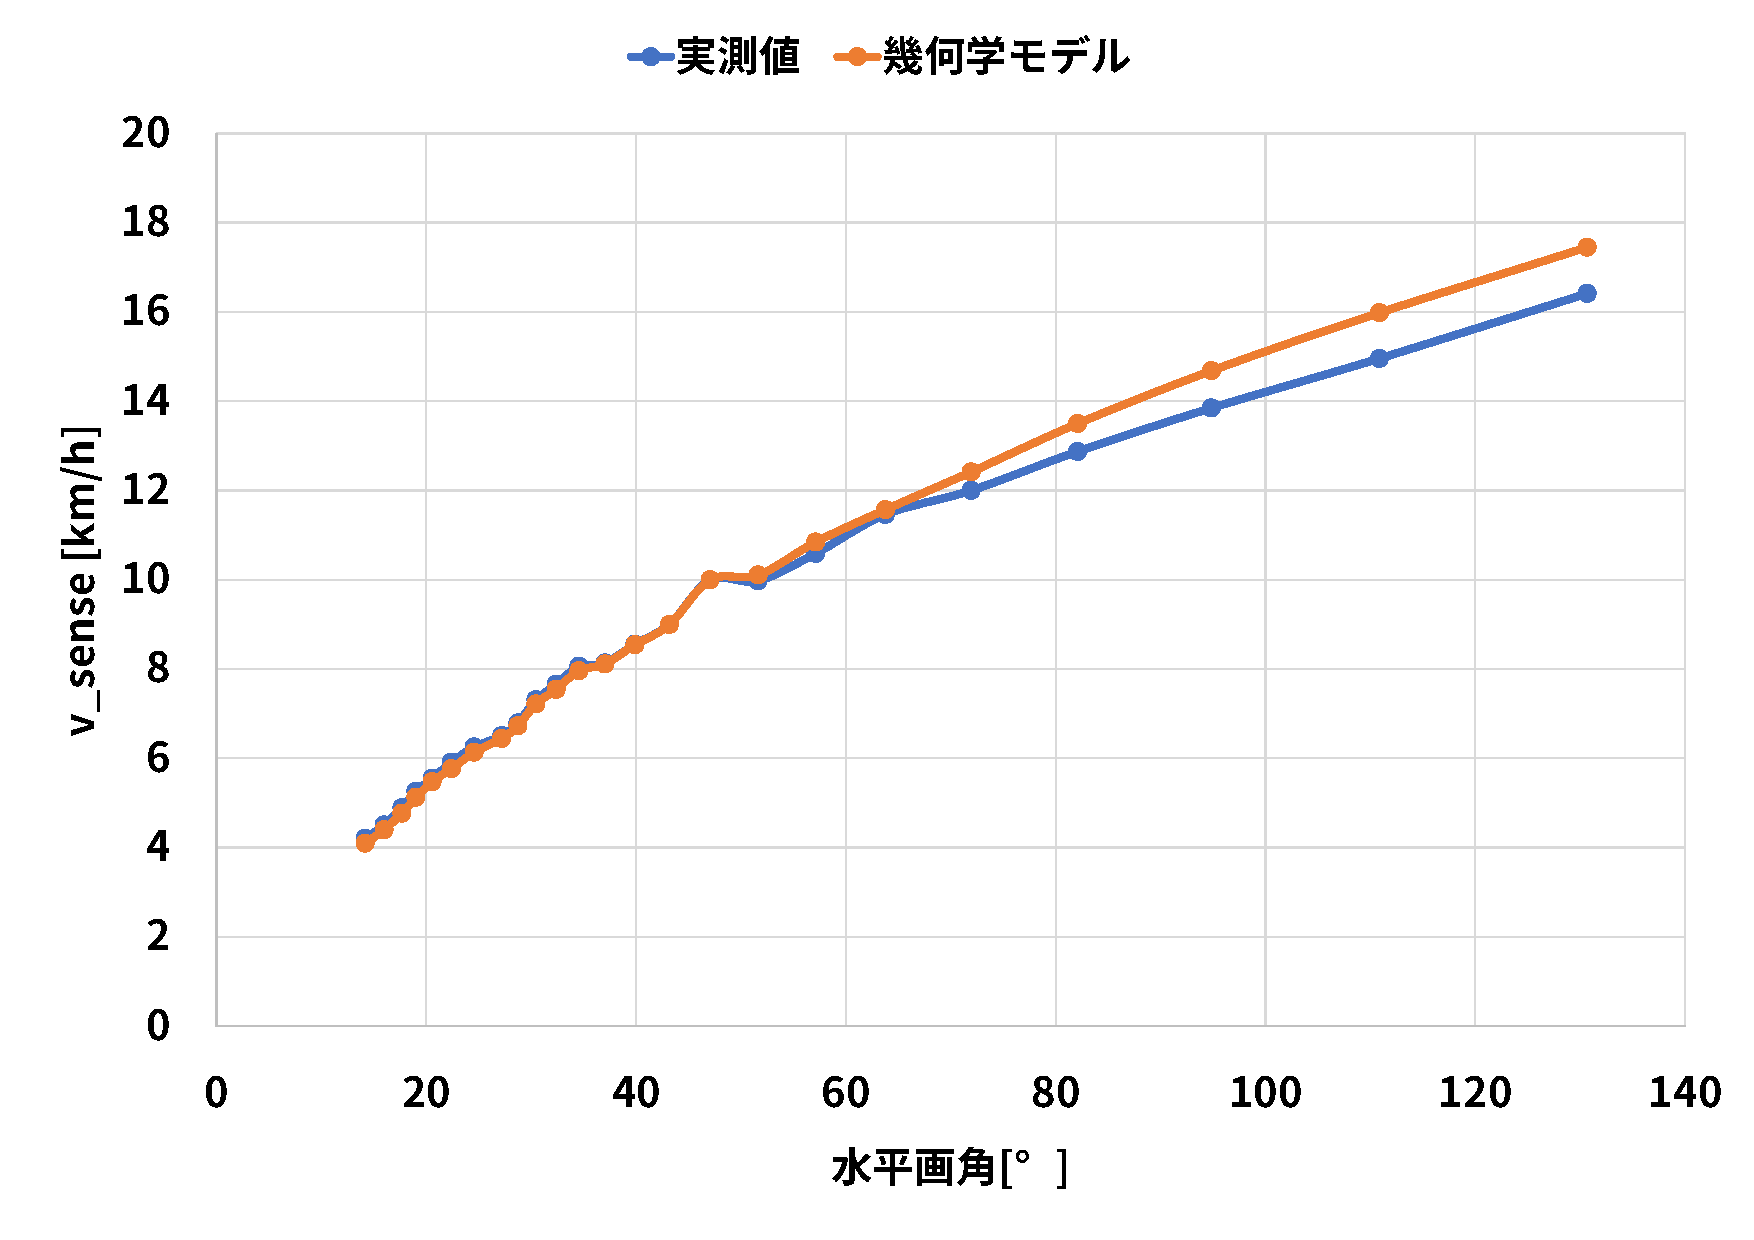
\includegraphics[width=.45\linewidth]{img/19.pdf}
    \label{auto:taikan_tokusie_final1}
    }
    \subfigure[クロップ率と体感速度の特性]{
    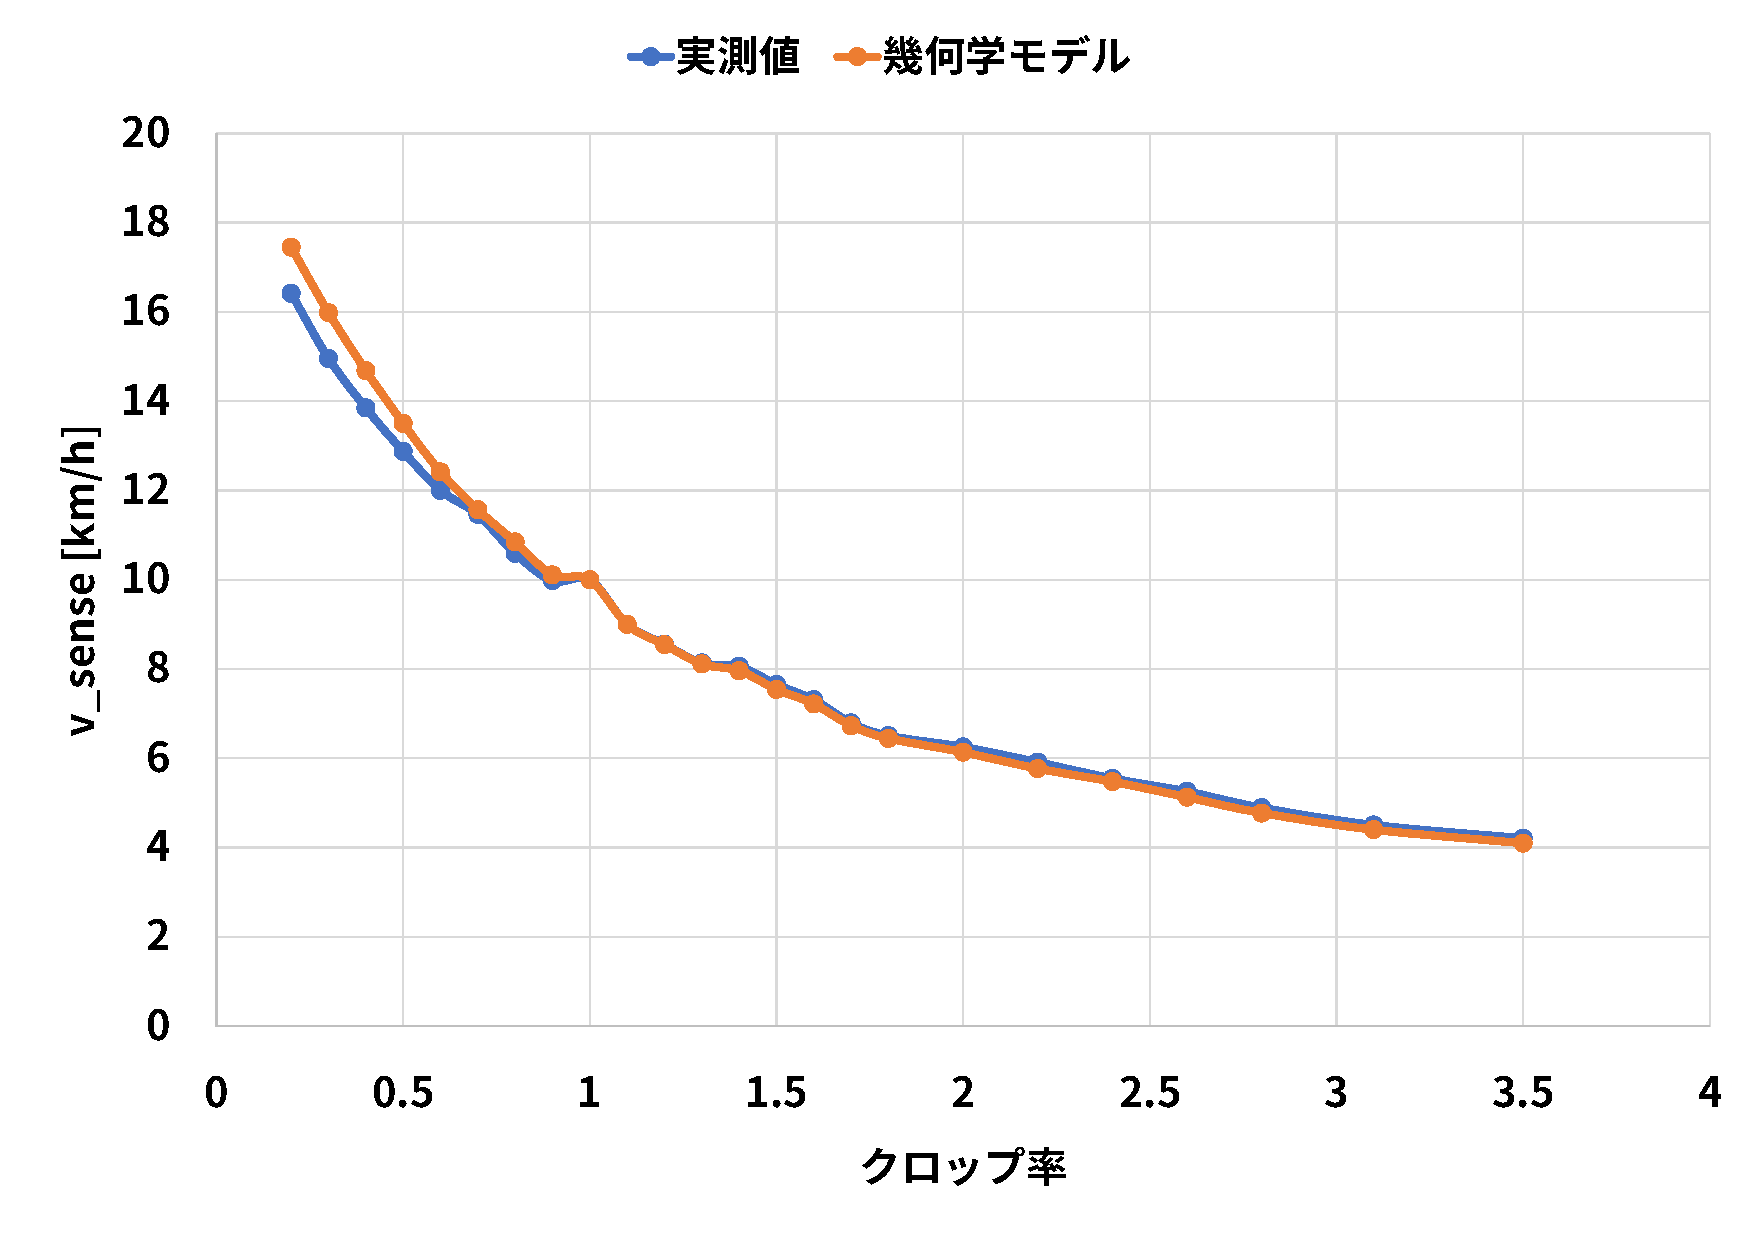
\includegraphics[width=.45\linewidth]{img/20.pdf}
    \label{auto:taikan_tokusei_final2}
    }
    \caption{体感速度モデル}
    \label{auto:taikan_tokusei_final}
  \end{center}
\end{figure}

第1章「序論」では研究背景として近年の自動運転システム・自律移動ロボットの研究開発を俯瞰し、
本研究が目指す遠隔型自動運転システムのユーザビリティの立ち位置、自律移動ロボットにおける実証実験の必要性、
自律移動ロボットの開発方針と、著者自身の研究の位置づけ・目標設定について述べた。

第2章「FPV車両操作の体感速度変化率の定式化」では、
体感速度の関連研究において、定性的な体感速度の変化について議論されている一方、
体感速度の定量化がなされていない点を取り上げ、
独自に、遠隔型自動運転システムのFPV操作に着目した、自動車の映像における運転視野角や、
映像画角の変化による体感速度のモデルの定量化を目的として、体感速度モデルの定式化を提案した。
成果として、体感速度はおおよそ視野角の根に比例する特性に近く、クロップ率に対して単調に減少する特性であるモデルを提案した。

第3章「LiDARのみのSLAMで作成された環境地図の評価」では、
ROSに実装されたSLAMメタパッケージである、GmappingとHector SLAMとCartographerによる環境地図構築システムを開発し、
LiDARのみによるSLAMによって作成された自律移動用環境地図の精度を比較した。
成果として、CartographerによるSLAMが最も歪みが少なく、追ってGmapping、Hector SLAMの順に精度が高いことが明らかになった。
しかし、Gmappingがノイズに強い点で、以降の自動運転システムに採用した。

第4章「自動運転システムの開発」では、
ステアリングコントローラによる、ハンドルフットペダル型インターフェースによる遠隔操作の
手動運転のユーザビリティの分析と、手動運転自動運転の切り替えシステムの開発を行った。
ROS\verb|(Robot Operating System)|を用いた遠隔操作による手動運転と、
SLAMとWaypoint Navigationを実装した手動運転・自動運転の切り替えシステムを開発した。
第3章で得た知見として、SLAMパッケージとして、Gmappingを採用し環境地図構築とNavigationメタパッケージである、
Navigation Stack を用いて、4輪車両型RCカーの自律移動システムを実現した。
Waypoint Navigationにより、中継目的地を経由して、最終目的地まで自律移動を行い、
最終目的地に到着した時点で、手動運転に切り替えることで、運転操作の引継ぎを実現するシステムを実現した。
成果として、一つ目に、若年層の手動操作におけるステアリングのカウンター操作の補助の必要性が明らかになった。
二つ目に、LiDARのみの自律移動ロボットシステムにおいて、手動・自動運転の切り替え操作が可能であった。
三つ目に、自律移動による切り返し操作が目標地点を分割することによって可能であり、
目標地点を1点のみの指定で切り返しに成功したシミュレーションとは異なる結果であることが明らかになった。

本研究の特徴は、
遠隔型自動運転システムの体感速度に関する特性を体系化している点と、
シミュレーションと実機による実験評価を実施し、シミュレーションと実機の両方による実証実験の必要性を提言している点
である。


従来の研究では、定性的な体感速度の効果に関する記述と、非常に高価な内界センサを用いたものである。
対して、我々の研究では、自律移動に関しては、LiDARのみと、1/10スケールのRCカーを用い、
比較的小規模で、安価でハードウェアの制約がある中で、シミュレーションと実機の両者を比較して
新たな手法へと発展させている研究は非常に少ない。

本研究は、遠隔型自動運転における体感速度のモデル化と、
安価なハードウェアにおける自律移動の妥当性を検証するための方法を提案することで、
移動ロボットの能力向上に大きく貢献したと信ずる。